\subsection{Merge sort}

\subsubsection{Ý tưởng}
Merge Sort là một thuật toán sắp xếp dựa trên phương pháp "chia để trị". Ý tưởng chính của thuật toán này là liên tục chia nhỏ mảng cần sắp xếp thành các mảng con nhỏ hơn cho đến khi mỗi mảng con chỉ còn một phần tử (đã được sắp xếp). Sau đó, các mảng con này được hợp nhất lại với nhau một cách có thứ tự để tạo thành mảng đã sắp xếp.

Quá trình hoạt động của Merge Sort bao gồm hai bước chính:
\begin{itemize}
    \item Chia: Mảng ban đầu được chia đều thành hai nửa. Quá trình chia này được lặp lại cho đến khi mỗi mảng con chỉ còn một phần tử.
    \item Trộn: Các mảng con được hợp nhất lại thành các mảng lớn hơn một cách có thứ tự. Trong quá trình hợp nhất, các phần tử của hai mảng con được so sánh và chèn vào mảng kết quả theo thứ tự tăng dần (hoặc giảm dần).
\end{itemize}
    
\subsubsection{Các bước hoạt động}
Xét mảng A như sau: 
\begin{center}
   A = \{38, 27, 43, 3, 9, 82, 10\} 
\end{center} 

\textbf{Các bước thực hiện:}

\begin{enumerate}
    \item \textbf{Chia đôi mảng:}
    \begin{itemize}
        \item Chia \( A \) thành hai nửa, với \( L \) nhiều phần tử hơn:
        \[
        L = \{38, 27, 43, 3\}, \quad R = \{9, 82, 10\}.
        \]
        \item Tiếp tục chia đệ quy:
        \[
        L \rightarrow \{38, 27\}, \{43, 3\}, \quad R \rightarrow \{9, 82\}, \{10\}.
        \]
        \item Lặp lại đến khi mỗi mảng chỉ còn một phần tử:
        \[
        L = \{38\}, \{27\}, \{43\}, \{3\}, \quad R = \{9\}, \{82\}, \{10\}.
        \]
    \end{itemize}
    
    \item \textbf{Trộn hai mảng đã sắp xếp:}
    \begin{itemize}
        \item So sánh các phần tử và trộn lại:
        \[
        \{38\}, \{27\} \rightarrow \{27, 38\}, \quad \{43\}, \{3\} \rightarrow \{3, 43\}.
        \]
        \item Tiếp tục:
        \[
        \{27, 38\}, \{3, 43\} \rightarrow \{3, 27, 38, 43\}, \quad \{9\}, \{82\} \rightarrow \{9, 82\}.
        \]
        \item Trộn nửa lớn hơn:
        \[
        \{9, 82\}, \{10\} \rightarrow \{9, 10, 82\}.
        \]
        \item Cuối cùng:
        \[
        \{3, 27, 38, 43\}, \{9, 10, 82\} \rightarrow \{3, 9, 10, 27, 38, 43, 82\}.
        \]
    \end{itemize}

    \item \textbf{Mảng kết quả:}
    Mảng đã sắp xếp:
    \[
    A = \{3, 9, 10, 27, 38, 43, 82\}.
    \]

\end{enumerate}


\begin{figure}[H]
    \centering
    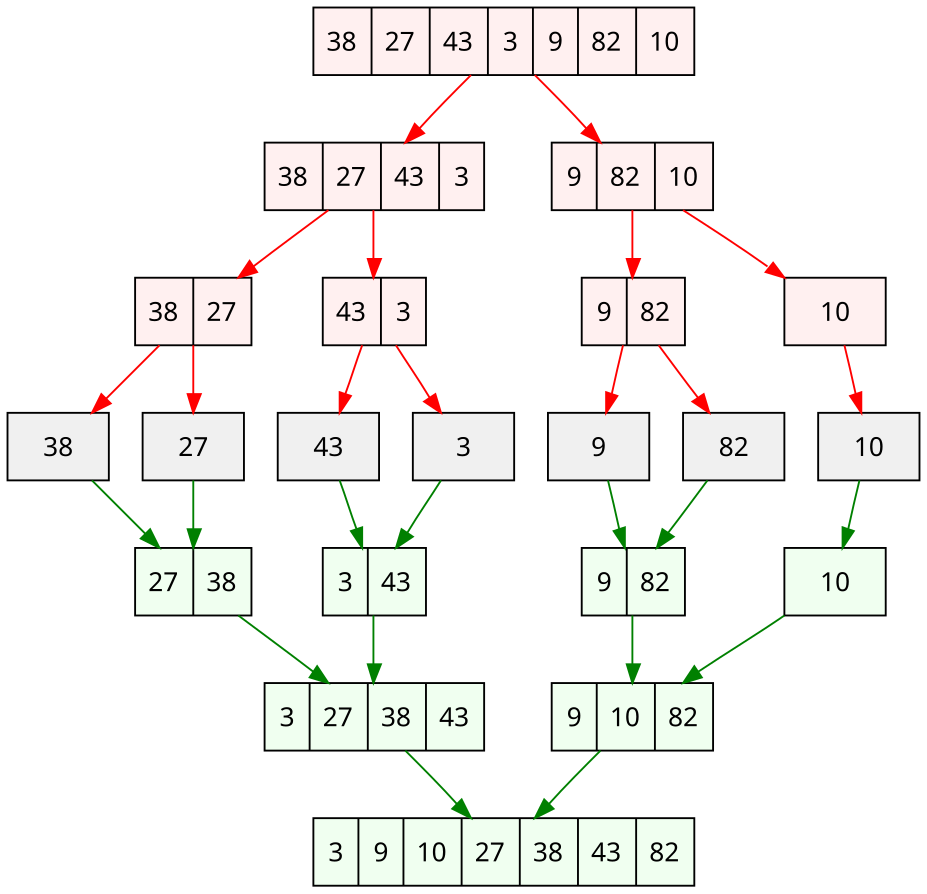
\includegraphics[width=0.8\textwidth]{img/Merge_sort_algorithm_diagram.svg.png}
    \caption{\href{https://en.wikipedia.org/wiki/File:Merge_sort_algorithm_diagram.svg.png}{Merge Sort Algorithm Diagram}}
\end{figure}

\subsubsection{Mã giả}
 
\begin{algorithm}[H]
\caption{Merge Sort}
\label{alg:merge-sort}
\begin{algorithmic}

\Require $A$ is an array of size $n$

\Function {merge}{\textit{A}, \textit{left}, \textit{mid}, \textit{right}}
\State Create temporary arrays $L$ and $R$
\State Copy $A[left \dots mid]$ into $L$, and $A[mid+1 \dots right]$ into $R$
\State Merge $L$ and $R$ back into $A$
\EndFunction \State

\Function {merge-sort}{\textit{A}, \textit{left}, \textit{right}}
\If{$left < right$}
    \State $mid \gets \lfloor (left + right) / 2 \rfloor$ \State
    \Call{merge-sort}{A, left, mid} \Comment{Sort the left half} \State
    \Call{merge-sort}{A, mid+1, right} \Comment{Sort the right half} \State
    \Call{merge}{A, left, mid, right} \Comment{Merge the two halves}
\EndIf
\EndFunction

\end{algorithmic}
\end{algorithm}


\subsubsection{Độ phức tạp}
\textbf{Độ phức tạp thời gian}

\footnote{Chương 7, Merge Sort, trang 307 \cite{dsa-analysis-cpp}} Gọi $T(n)$ là thời gian thực hiện của thuật toán khi được áp dụng lên một dãy dữ liệu có kích thước $n$.
Giả sử $n$ là một lũy thừa của 2 (n có dạng $2^k$ với $k \in \mathbb{N}^*$), do đó luôn chia mảng ban đầu thành 2 nửa chẵn. Với $n = 1$, thời gian sắp xếp của Merge Sort là hằng số, kí hiệu là 1. Mặt khác, thời gian thực hiện Merge Sort cho $n$ số bằng thời gian thực hiện hai phép sắp xếp hợp nhất đệ quy có kích thước n/2, cộng với thời gian để hợp nhất, là tuyến tính. 

Các phương trình sau đây nói chính xác điều này:

$$\left\{
\begin{array}{l}
        T(1) = 1 \\
        T(n) = T(\frac{n}{2}) + n
\end{array}
\right.$$

Đây là một quan hệ đệ quy chuẩn, có thể được giải theo nhiều cách. Bài báo cáo này sẽ trình bày hai phương pháp. Ý tưởng đầu tiên là chia quan hệ đệ quy cho n. Điều này tạo ra

$$\frac{T(n)}{n} = \frac{T(n / 2)}{n / 2} + 1$$

Phương trình này hợp lệ với bất kỳ n nào là lũy thừa của 2, vì vậy chúng ta cũng có thể viết 

\begin{align*}
    \frac{T(n/2)}{n/2} &= \frac{T(n / 4)}{n / 4} + 1 \\
    \frac{T(n/4)}{n/4} &= \frac{T(n / 8)}{n / 8} + 1 \\
    \dots \\
    \frac{T(2)}{2} &= \frac{T(1)}{1} + 1
\end{align*}

Bây giờ cộng tất cả các phương trình lại. Điều này có nghĩa là cộng tất cả các số hạng ở vế trái và đặt kết quả bằng tổng của tất cả các số hạng ở vế phải. Lưu ý rằng số hạng $T(n/2)/(n/2)$ xuất hiện ở cả hai vế và do đó triệt tiêu. Trên thực tế, hầu như tất cả các số hạng xuất hiện ở cả hai vế và triệt tiêu. Sau khi mọi thứ được cộng lại, kết quả cuối cùng là 

$$\frac{T(n)}{n} = \frac{T(1)}{1} + \log{n}$$

Vì tất cả các số hạng khác triệt tiêu và có $\log{n}$ phương trình, do đó tất cả các số 1 ở cuối các phương trình này cộng lại bằng $\log{n}$. Nhân qua n sẽ cho kết quả cuối cùng. 

$$T(n) = n +  n\log{n}$$

Một phương pháp thay thế là thay thế mối quan hệ đệ quy liên tục ở vế phải.

Ta có 
$$T(n) = 2T(n/2) + n$$

Thay $n/2$ vào phương trình chính:

\begin{align*}
    2T(n/2) &= 2(2T(n/4) + n / 2) = 4T(n/4) + n \\
    \Rightarrow T(n) &= 4T(n / 4) + 2n
\end{align*}

Một lần nữa, bằng cách thay thế $n/4$ vào phương trình chính, ta thấy rằng 

\begin{align*}
    4T(n/4) &= 4(2T(n/8) + n / 4) = 8T(n/8) + n \\
    \Rightarrow T(n) &= 8T(n / 8) + 3n
\end{align*}

Tiếp tục theo cách này, ta thu được

$$T(n) = 2^kT(n/2^k) + kn$$


Sử dụng $k = \log{n}$, ta thu được

$$T(n) = nT(1) + n\log{n} = n\log{n} + n$$

Kết luận về độ phức tạp thời gian:

 \begin{itemize}
    \item Trường hợp tốt nhất: $\Omega(n\log{n})$ 
    \item Trường hợp xấu nhất: $O(n\log{n})$
    \item Trường hợp trung bình: $\Theta(n\log{n})$
\end{itemize}

\textbf{Độ phức tạp không gian}

Trong bước trộn hai dãy con của Merge Sort có sử dụng mảng phụ để lưu tạm thời các giá trị nên chi phí không gian của giải thuật này là $O(n)$.

\subsubsection{Nhận xét}

Merge Sort là một thuật toán sắp xếp hiệu quả và ổn định, phù hợp với các trường hợp yêu cầu giữ nguyên thứ tự của các phần tử có giá trị bằng nhau. Tuy nhiên, việc sử dụng đệ quy có thể ảnh hưởng đến hiệu suất thực tế. 

\textbf{Cải tiến}

Một cách cải tiến đó là khử đệ quy (Iterative Merge Sort) giúp  giảm bộ nhớ sử dụng do không gọi đệ quy.